\documentclass{beamer}
\usepackage{apacite}
\usepackage{graphicx}

\usetheme{Frankfurt}
\graphicspath{{.}}
\setbeamertemplate{caption}[numbered]

% ornate: boadilla frankfurt
% simple: default montpellier singapore szeged34013833


\title{Linking the wealth of people and places}
\subtitle{Survey data and OpenStreetMap}
\author{Chandler Armstrong}
\institute{CERL}
\date{Spring 2018}


\bibliographystyle{apacite}


\begin{document}


\begin{frame}
\titlepage
\end{frame}


\begin{frame}{Agenda}
  \begin{itemize}
  \item The wealth of people \& places
  \item Benefits
  \item Challenges \& problems
  \end{itemize}
\end{frame}


\begin{frame}{Mapping wealth}  
  \begin{center}
    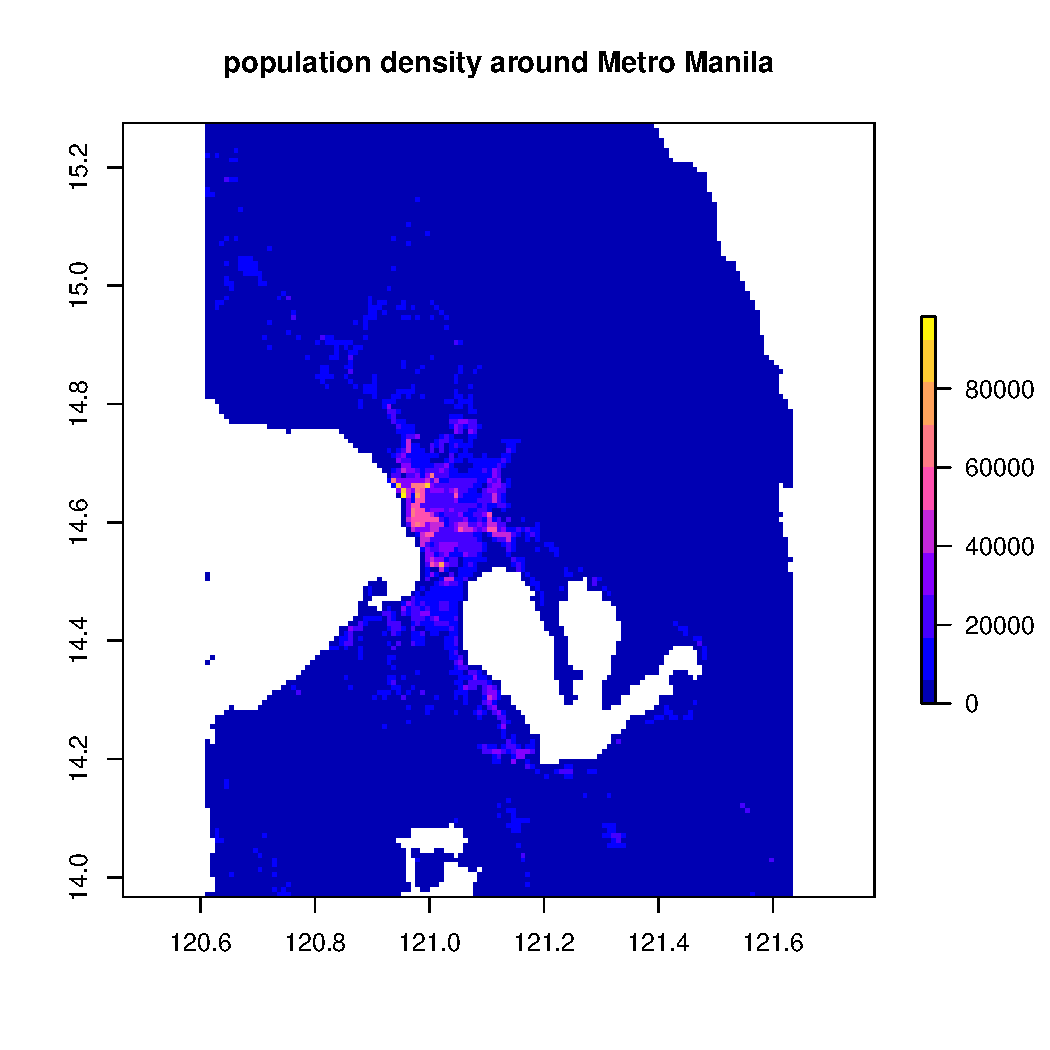
\includegraphics[width=0.4\textheight]{landscan}%
  \end{center}
  \begin{itemize}
  \item people-based (economic, human, \& social capital)
    \begin{itemize}
    \item social networks
    \item education
    \item bank account
    \end{itemize}
  \item place-based (natural, ecological, \& community capital)
    \begin{itemize}
    \item infrastructure (a dam, roads)
    \item natural resources (forest, wetlands)
    \item social services (banks, theatre, retail)
    \end{itemize}
  \end{itemize}
\end{frame}


\begin{frame}{Case: disaster-driven migration}
  \begin{description}
  \item[people-based] propensity to migrate
  \item[place-based] food \& water availability following a disaster
  \end{description}
Grocery stores are a critical source of lifesaving supplies during and after a disaster, however supply chains are often disrupted and unable to deliver the surge of supplies required by the population \cite{palin17}.  Following a disaster, certain types of non-perishable goods may remain sparsely available and out-of-stock for many months \cite{cavallo14}.
\end{frame}


\begin{frame}{Food \& water availability}
  \begin{figure}
  \begin{center}
    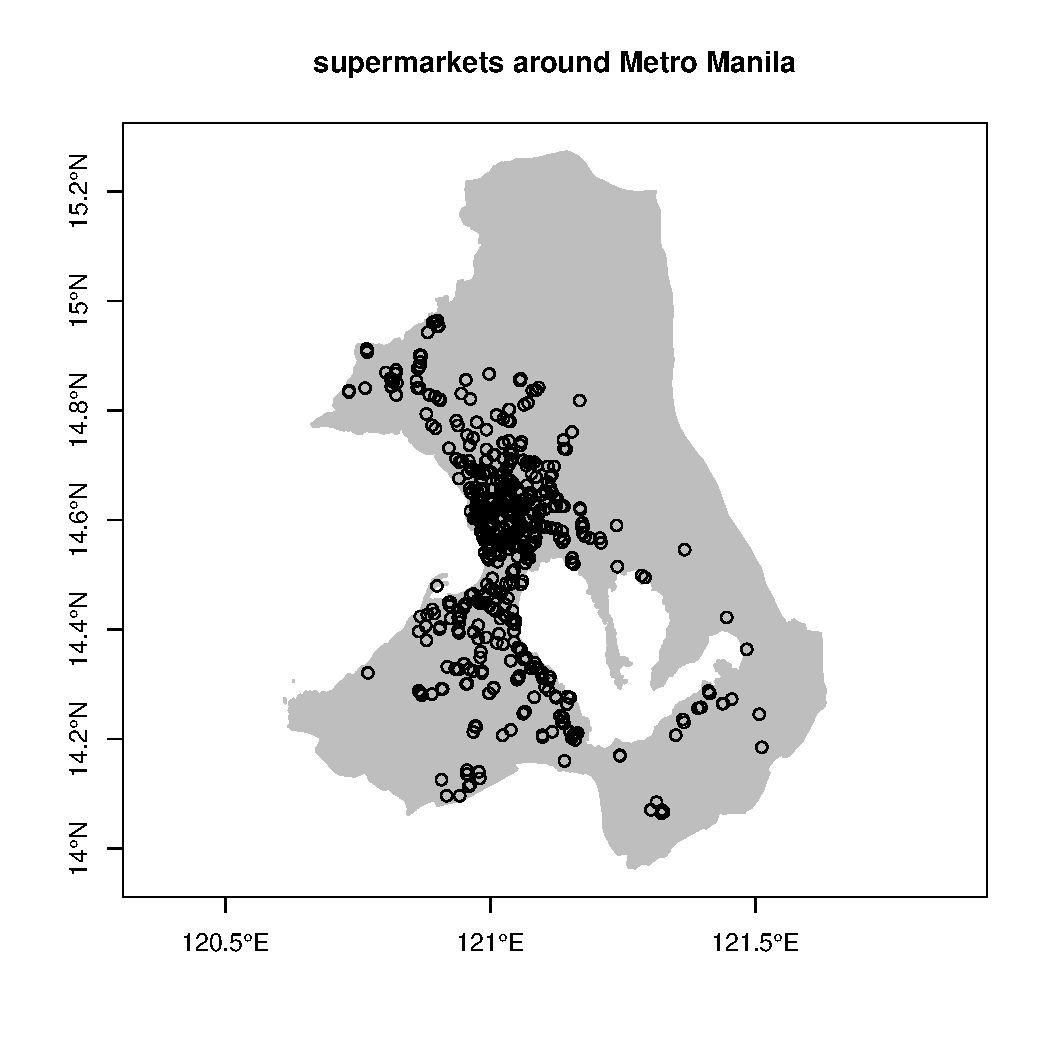
\includegraphics[width=0.3\textwidth]{supermarkets}%
    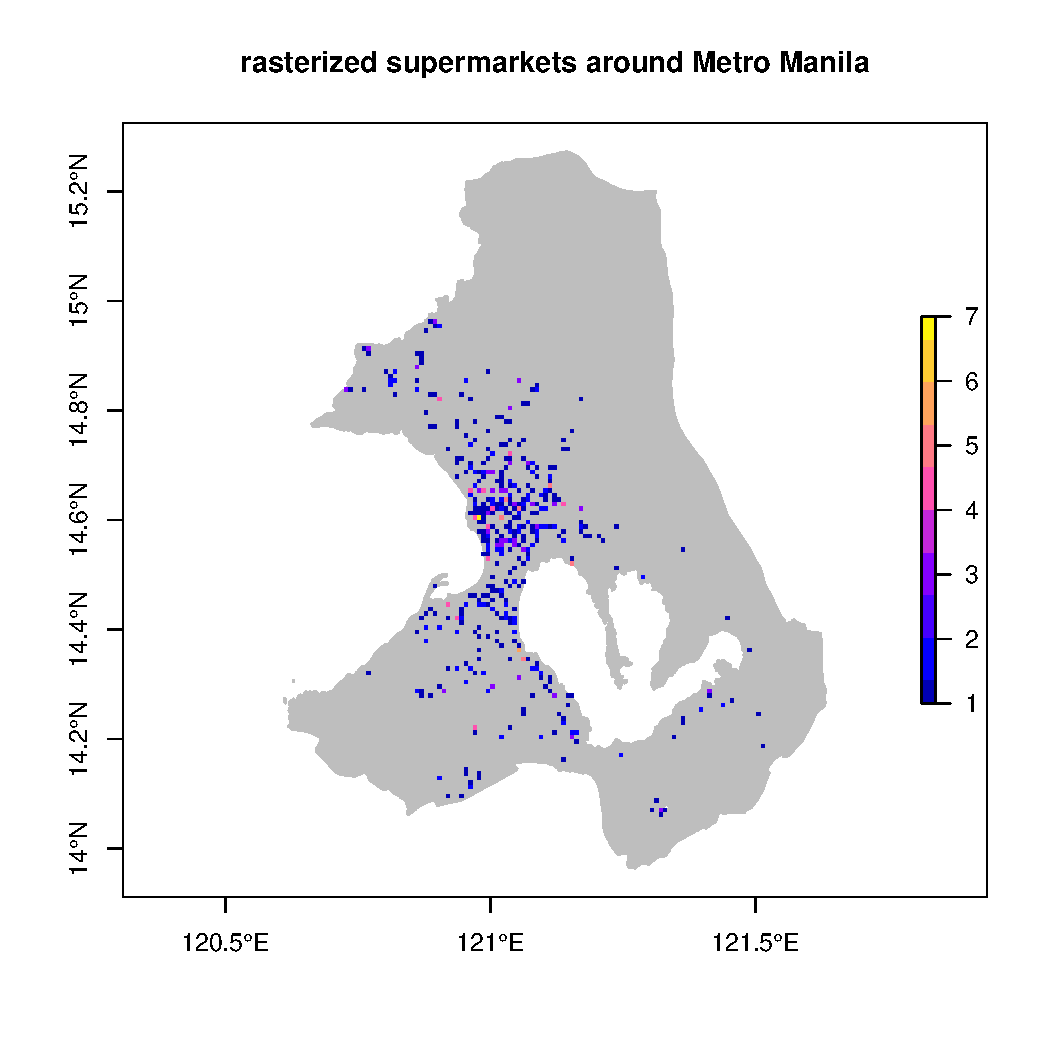
\includegraphics[width=0.3\textwidth]{rSupermarkets}%
    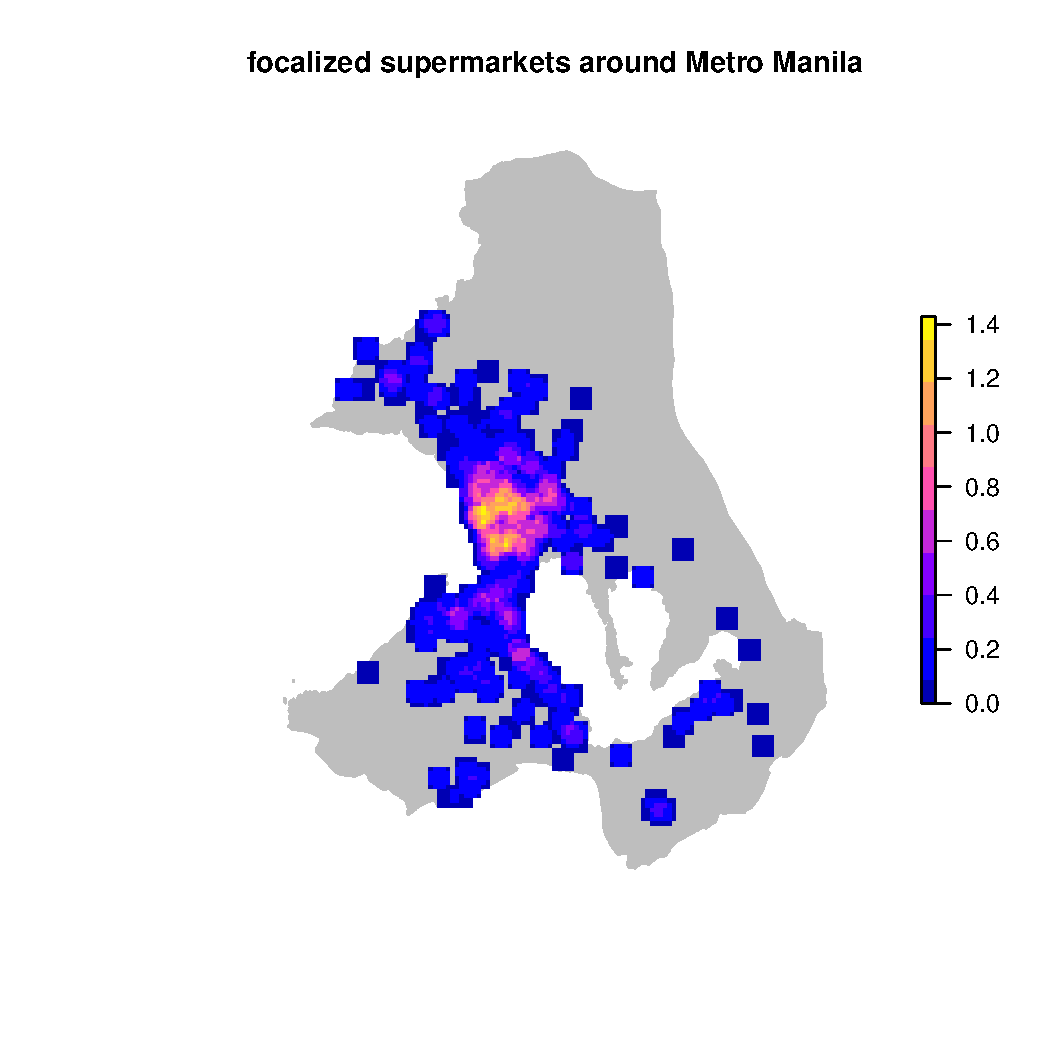
\includegraphics[width=0.3\textwidth]{rSupermarketsFocal}
    % summed into raster cells
  \end{center}
  \caption{\cite{openstreetmap}}
  \end{figure}
  % \begin{itemize}
  % \item supermarkets
  % \end{itemize}
\end{frame}


\begin{frame}{Propensity to migrate}
  \begin{itemize}
  \item past migration
  \item resources to migrate
  \item distance to potential immigration site
  \end{itemize}
  \begin{table}

  \begin{tabular}{l l l}
    \hline
    variable(1=`yes')  & mean(standard deviation) & n missing \\
    \hline
    migration, 5-year  & 0.031(0.03) & 1353467 \\
    migration, 10-year & 0.04(0.038) & 2280714 \\
    native             & 0.98(0.02) & 251850 \\
    % distance to home & & \\
    \hline
   \end{tabular}

  \caption{\cite{ipums}}
  \end{table}

\end{frame}


\begin{frame}{Dasymetric mapping \& population characterization}
  \begin{center}
    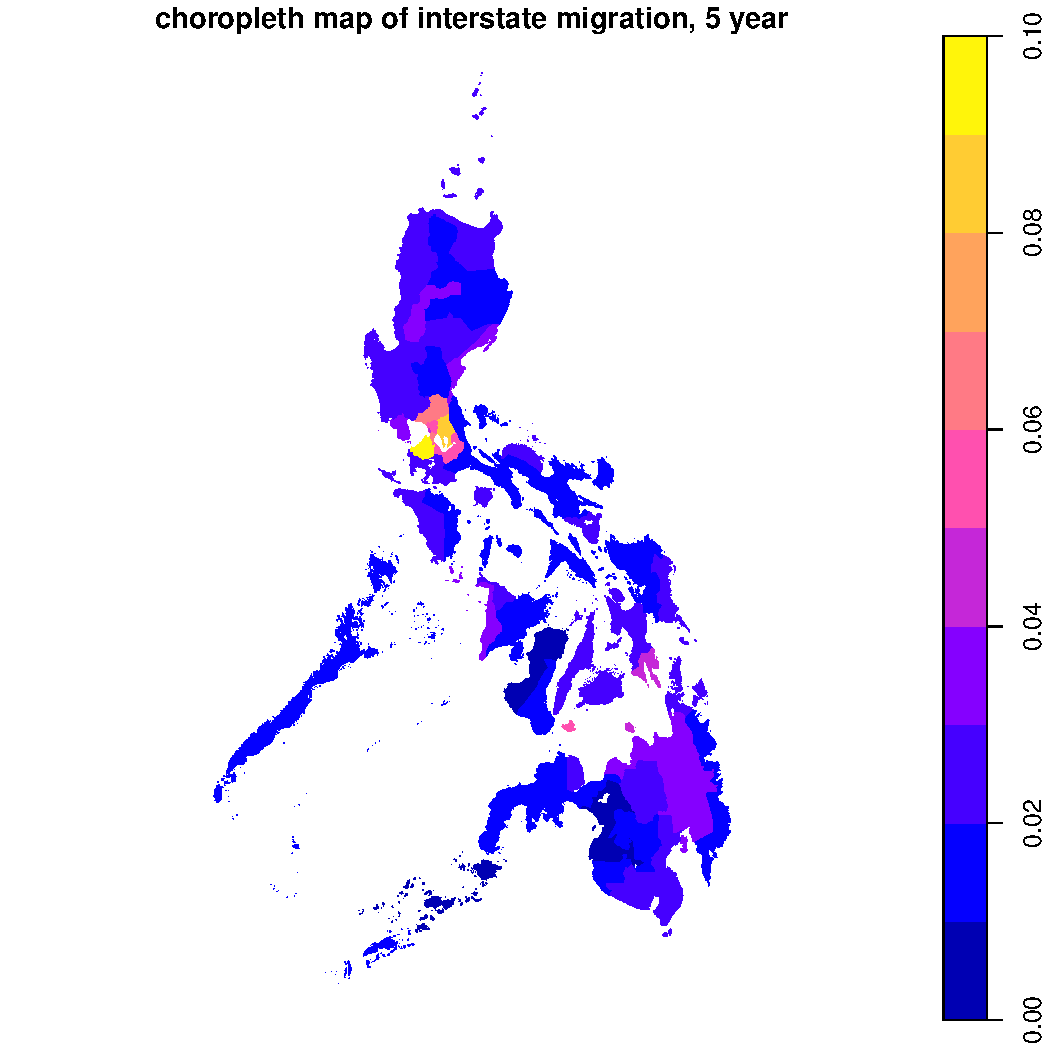
\includegraphics[width=0.3\textwidth]{choropleth}%
    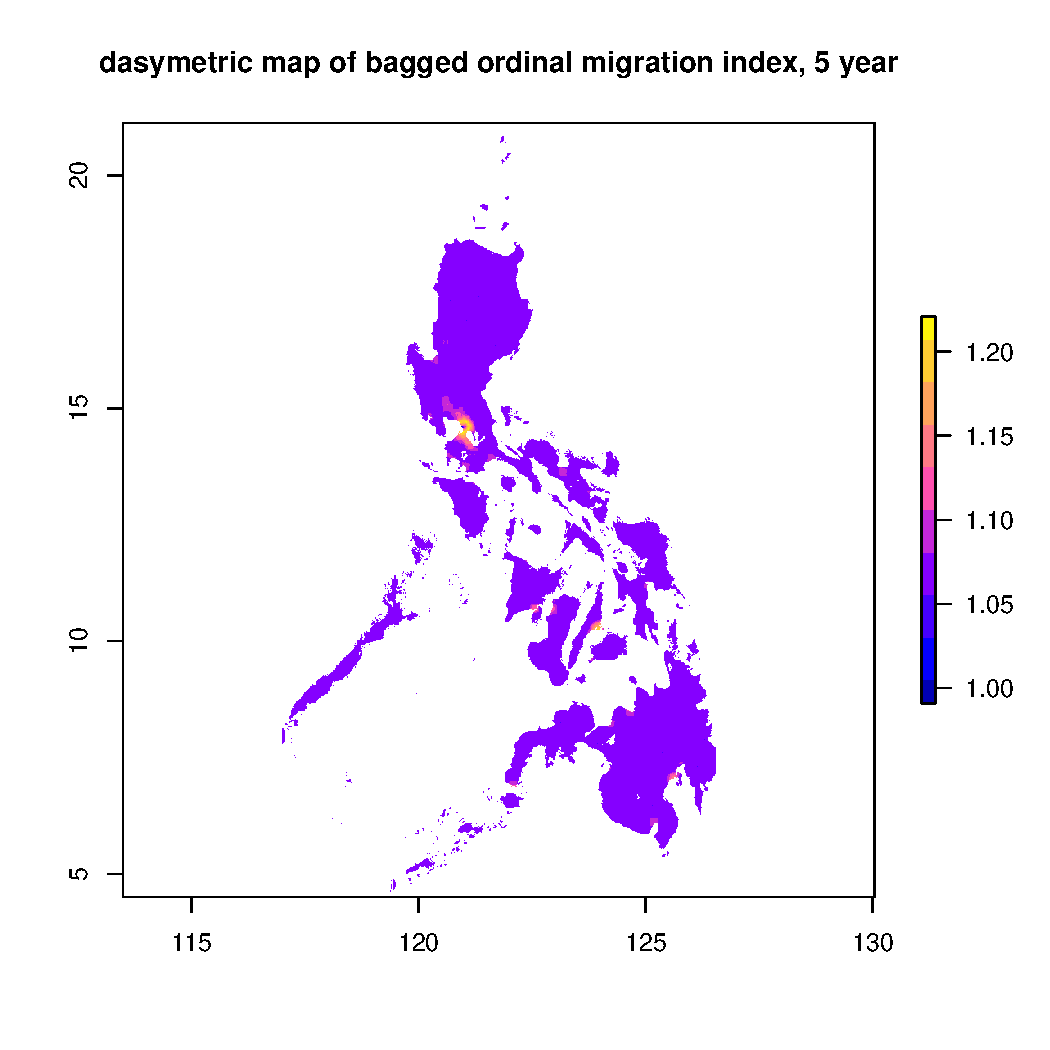
\includegraphics[width=0.3\textwidth]{dasymetric}%
    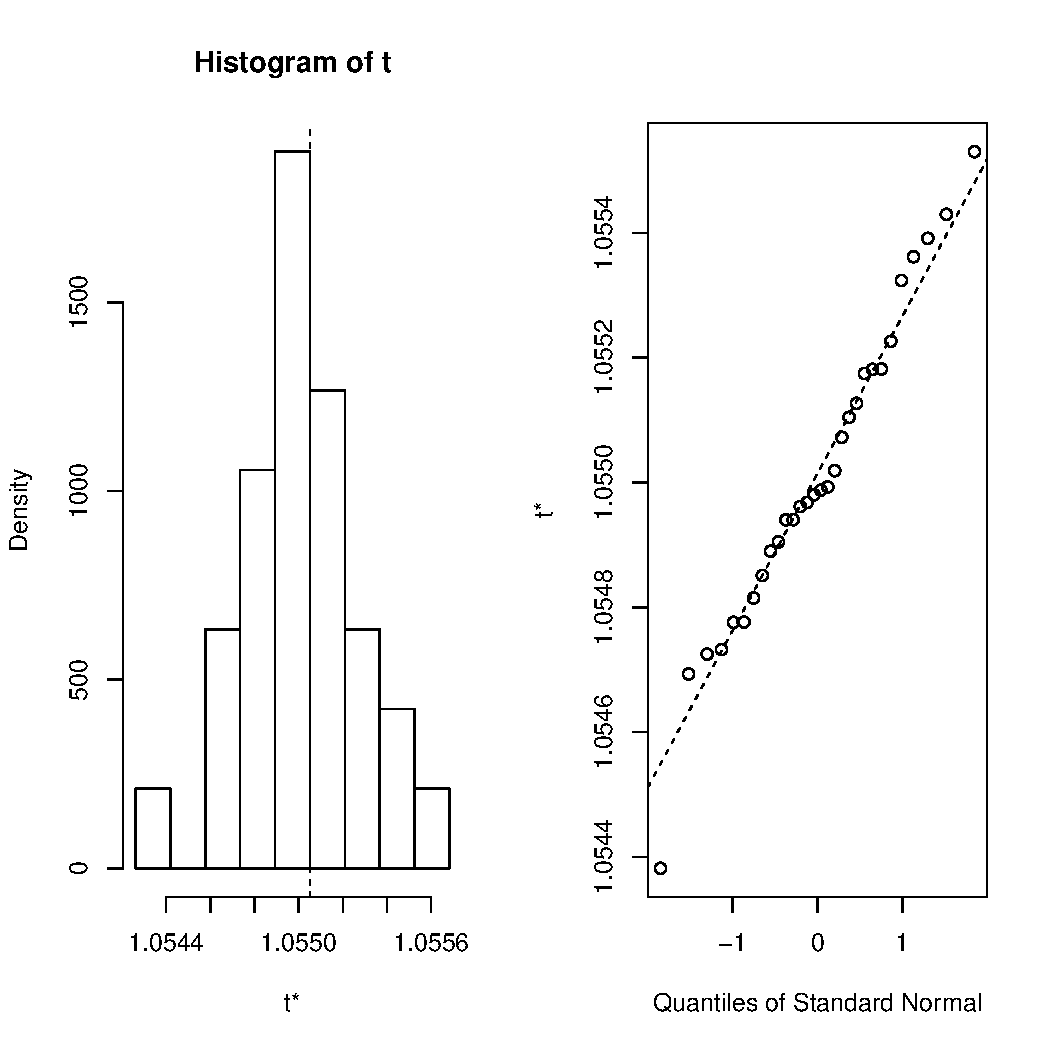
\includegraphics[width=0.3\textwidth]{bagged}
  \end{center}
  % The input population maps are themselves models:
  \begin{itemize}
  \item administrative population data
  \item landcover
  \item roads
  \item points
  \end{itemize}
  % The output of one dasymetric map can be input to another
\end{frame}


\begin{frame}{Linking the wealth of people \& places}
  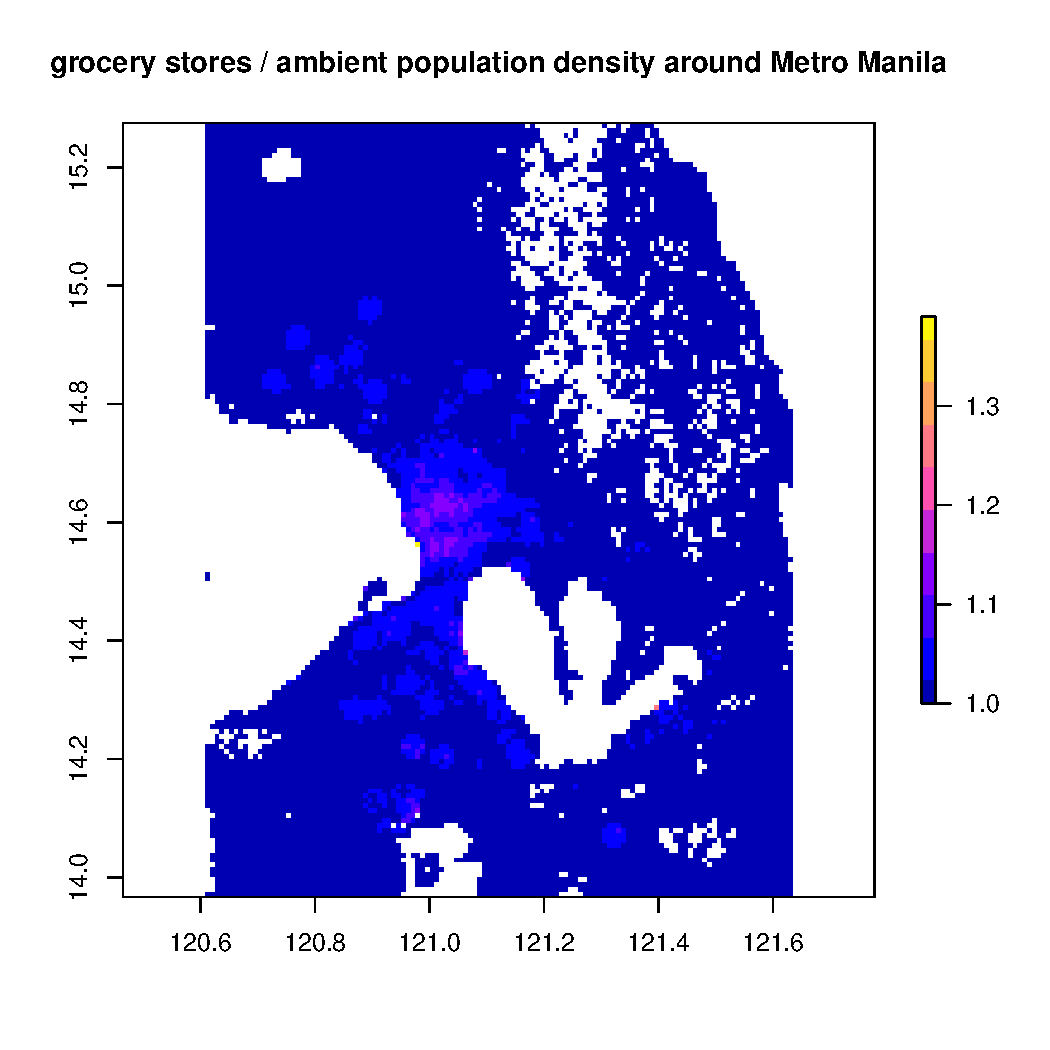
\includegraphics[width=0.3\textwidth]{rSupermarketsFocalNorm}% +
  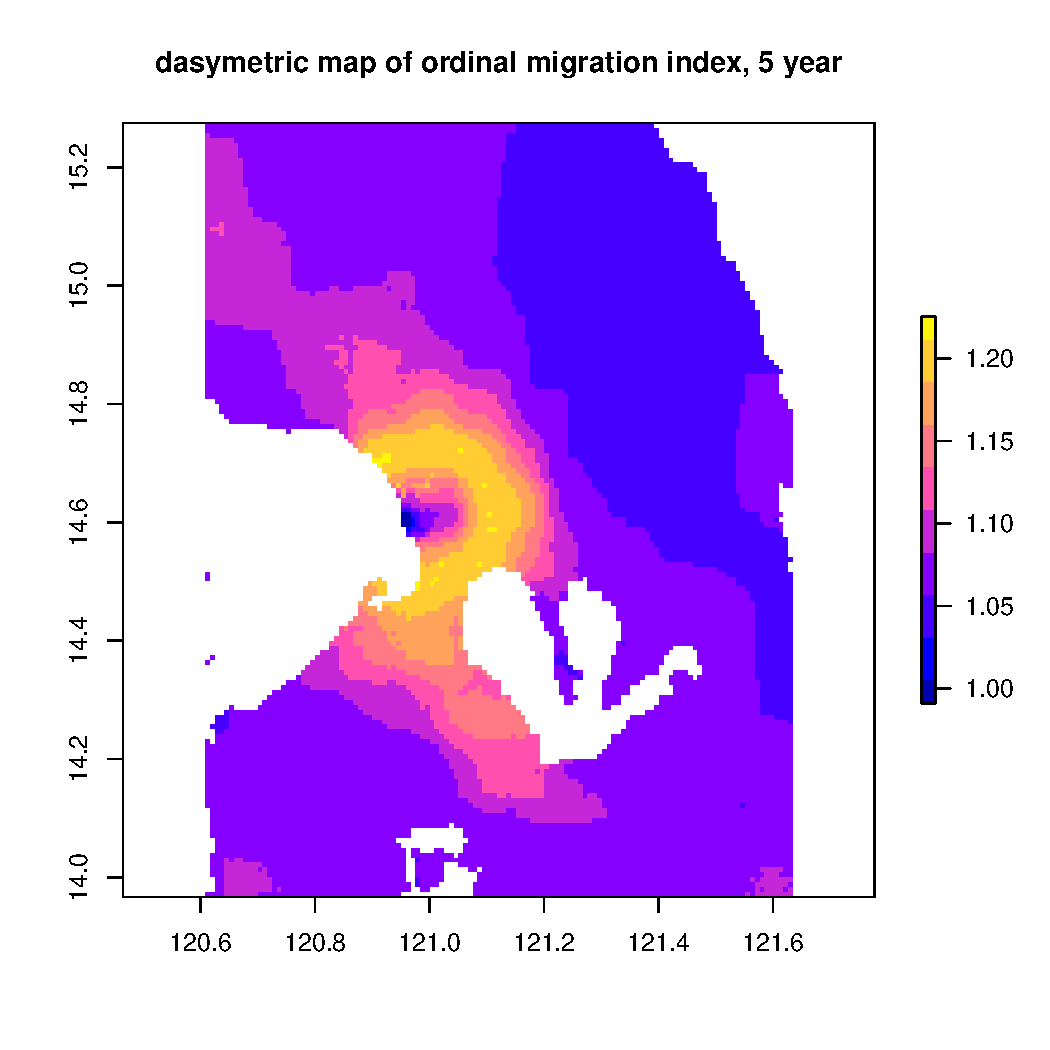
\includegraphics[width=0.3\textwidth]{dasymetricMM}%
  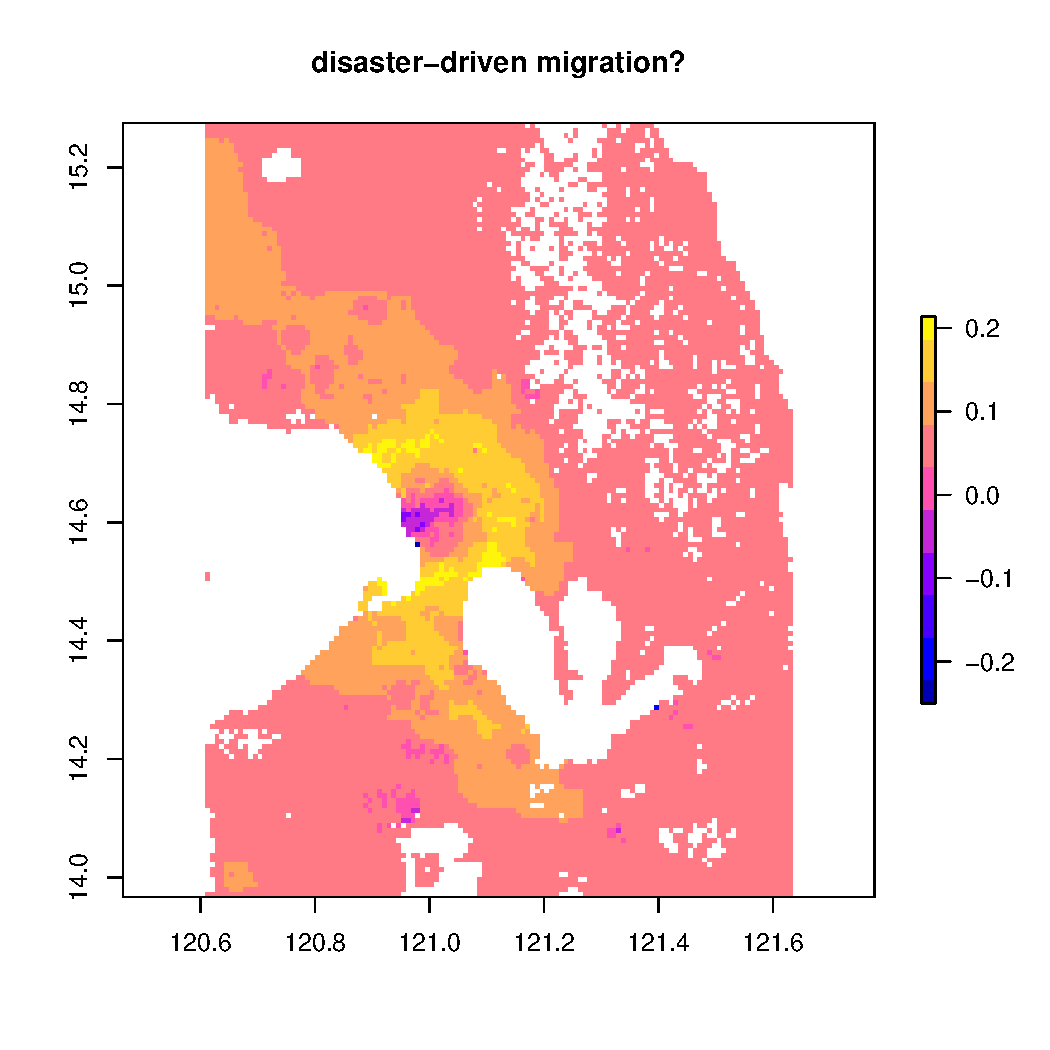
\includegraphics[width=0.3\textwidth]{disaster_driven}
\end{frame}

% \begin{frame}{Research questions}
% \begin{enumerate}
%   \item How do models producing input data influence the output?
%   \item How to include spatial dependence?
%   \item How to incorporate (dirty) point data?
%   \item What does it all mean?
% \end{enumerate}
% \end{frame}


% \begin{frame}{Modelling effects}
%   \begin{center}
%     \includegraphics[height=0.5\textheight]{pop}%
%   \end{center}
%   The input population maps are themselves models:
%   \begin{itemize}
%   \item administrative population data
%   \item landcover
%   \item etc.
%   \end{itemize}
%   How to characterize that relationship?
%   \begin{itemize}
%   \item uncertainty
%   \item multiple equation model
%   \end{itemize}
%   $\Xhat=Z\delta_z+X\delta_x$
%   $\Yhat=\Xhat\Beta+X\Beta$
% \end{frame}


\begin{frame}{Challenges \& Problems}
  \begin{center}
    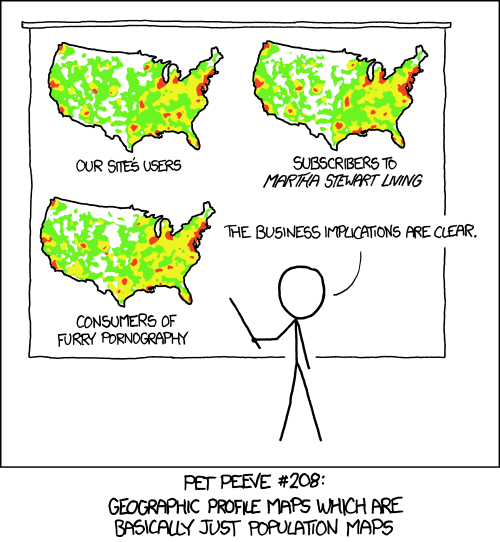
\includegraphics[width=0.4\textheight]{heatmap}
  \end{center}
  \begin{itemize}
  \item Population dominates
  \item Modifiable areal unit problem
  \item Embarrasingly parallel, but high space complexity
  \item Largely deductive, with little to no inductive validation
  \end{itemize}
\end{frame}


% disaster preparedness and mitigation, emergency responses, disaster rehabilitation and reconstruction.
\begin{frame}{Benefits}
  \begin{itemize}
  \item Re-expresses all data into a common format and resolution: easy analysis
  \item Simple to add new data to analysis: resampling \& aggregation
  \item Nonparametric: fast, fewer assumptions, analyze bias, skew, \& uncertainty
  \item Mapped demographics permit geospatial operations: distances, intersections, buffers, etc.
  \item Many applications: disaster preparedness \& mitigation, response, rehabilitation \& reconstruction
  \end{itemize}
\end{frame}
% overlay disaster data or modelled outputs with a characterized population raster and analyze how the affected population can respond through movement or other response strategies.  So, if a certain area of population is affected by water shortages, how far will people travel to obtain what they need?  Do they move to a location with more water, or do they stay and deal with less or lower quality water?  What is the threshold for water availability and quality where people decide to pack up and leave, resulting in disaster driven migration?


\bibliography{disasters}


\begin{frame}{POC}
\begin{description}
  \item[Chandler Armstrong, PI] chandler.m.armstrong@erdc.dren.mil
\end{description}
\end{frame}


\end{document}

%disconcerting conclusion that absent economic motivation ethnic diversity can still lead to violence.  BGD may not generalize well due to relative ethnic homogeneity.  Districts with greater diversity are uncommon and a little diversity in this situation may create tense environments.  It may also be that omitted variables exist correlated with both diversity and violence.  For example access to legitimate political power.

% model indegeneity
% kernel density of fractionalization

% ethnic diversity is really quite rare in BGD, and where it does occur something important may be happening to make these areas, in particular, more violent.  It may not be related to diversity, per se, but to the existence of a particular ethnicity, perhaps an indigenous one.

%%% Local Variables:
%%% mode: latex
%%% TeX-master: t
%%% End:
